\documentclass[a4paper,11pt,twocolumn]{article}
\usepackage[a4paper,left=1.5cm,right=1cm,top=2cm,bottom=2cm]{geometry}
\usepackage{setspace}
\usepackage{gensymb}
\usepackage{caption}
\usepackage{graphicx}
\usepackage{tabularx}
\usepackage{lmodern}
\usepackage{watermark} 
\usepackage{lipsum}
\usepackage{xcolor}
\usepackage{listings}
\usepackage{graphicx}
\usepackage{enumitem}
\usepackage{mathtools}
\usepackage{titlesec}
\usepackage[utf8]{inputenc}
\usepackage{fontenc}
\usepackage{harvard}
\usepackage{amsfonts}
\usepackage{tikz}
\graphicspath{{/storage/emulated/0/Download/FWC/Latex/figs}}
\usepackage[colorlinks,linkcolor={black},citecolor={blue!80!black},urlcolor={blue!80!black}]{hyperref}
\title{\textbf{\textsc{VERIFICATION OF XOR GATE}}}
\author{\textbf{\textit{\teflipflopxtbf{RAMESHWAR SAINATH PAWAR (1032222095)}}}}
\begin{document}
\date{}
\maketitle
\tableofcontents
\section{PROBLEM}
\textbf{(GATE CS-2OO2)}
\textbf{Q.12} Minimum sum of product expression for f(w,x,y,z) shown in Karnaugh-map below is

\tikzset{every picture/.style={line width=0.75pt}} %set default line width to 0.75pt        

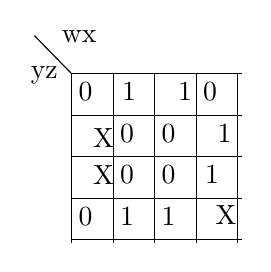
\begin{tikzpicture}[x=0.75pt,y=0.75pt,yscale=-1,xscale=1]
%uncomment if require: \path (0,235); %set diagram left start at 0, and has height of 235

%Shape: Grid [id:dp9981783189121591] 
\draw  [draw opacity=0] (106,41) -- (188,41) -- (188,122.6) -- (106,122.6) -- cycle ; \draw   (106,41) -- (106,122.6)(126,41) -- (126,122.6)(146,41) -- (146,122.6)(166,41) -- (166,122.6)(186,41) -- (186,122.6) ; \draw   (106,41) -- (188,41)(106,61) -- (188,61)(106,81) -- (188,81)(106,101) -- (188,101)(106,121) -- (188,121) ; \draw    ;
%Straight Lines [id:da6508935575311161] 
\draw    (88,22.6) -- (106,41) ;

% Text Node
\draw (169,84) node [anchor=north west][inner sep=0.75pt]   [align=left] {1};
% Text Node
\draw (156,44) node [anchor=north west][inner sep=0.75pt]   [align=left] {1};
% Text Node
\draw (175,64) node [anchor=north west][inner sep=0.75pt]   [align=left] {1};
% Text Node
\draw (129,44) node [anchor=north west][inner sep=0.75pt]   [align=left] {1};
% Text Node
\draw (115,66) node [anchor=north west][inner sep=0.75pt]   [align=left] {X};
% Text Node
\draw (115,84) node [anchor=north west][inner sep=0.75pt]   [align=left] {X};
% Text Node
\draw (174,103) node [anchor=north west][inner sep=0.75pt]   [align=left] {X};
% Text Node
\draw (100,19) node [anchor=north west][inner sep=0.75pt]   [align=left] {wx};
% Text Node
\draw (85,36) node [anchor=north west][inner sep=0.75pt]   [align=left] {yz};
% Text Node
\draw (148,104) node [anchor=north west][inner sep=0.75pt]   [align=left] {1};
% Text Node
\draw (128,104) node [anchor=north west][inner sep=0.75pt]   [align=left] {1};
% Text Node
\draw (108,104) node [anchor=north west][inner sep=0.75pt]   [align=left] {0};
% Text Node
\draw (128,84) node [anchor=north west][inner sep=0.75pt]   [align=left] {0};
% Text Node
\draw (148,84) node [anchor=north west][inner sep=0.75pt]   [align=left] {0};
% Text Node
\draw (148,64) node [anchor=north west][inner sep=0.75pt]   [align=left] {0};
% Text Node
\draw (128,64) node [anchor=north west][inner sep=0.75pt]   [align=left] {0};
% Text Node
\draw (108,44) node [anchor=north west][inner sep=0.75pt]   [align=left] {0};
% Text Node
\draw (168,44) node [anchor=north west][inner sep=0.75pt]   [align=left] {0};
\end{tikzpicture}
\end{tikzpicture}
\begin{enumerate}[label=(\Alph*)]
	\item $ x&&z+y'&&z$
	\item $ x&&z'+z&&x'$
	\item $ x'&&y+z&&x'$
	\item $ None of the above $
\end{enumerate}
\bigskip
\section{COMPONENTS}
	\begin{tabularx}{0.45\textwidth} {  
  | >{\centering\arraybackslash}X  
  | >{\centering\arraybackslash}X  
  | >{\centering\arraybackslash}X | } 
\hline 
\textbf{Component} &  \textbf{Value} & \textbf{Quantity}\\ 
\hline 
Arduino & UNO & 1 \\   
\hline 
Bread board & - & 1 \\ 
\hline 
IC & - & - \\
\hline
Jumper wires & M-M & 20 \\ 
\hline 
LED  & - & -\\ 
\hline 
Resistor & 150ohms & 1\\ 
\hline 
\end{tabularx}
\bigskip
\section{INTRODUCTION}
\paragraph{}
	the problem involves simplifying a Boolean function using a Karnaugh map. We need to identify groups of adjacent 1s in the map and use them to create the simplest sum of product (SOP) expression that represents the function. The goal is to choose the correct expression from the provided options that accurately represents the function's simplified form 
\bigskip 
\section{TRUTH TABLE}
The Truth Table for the above identities is ass follows:
\tikzset{every picture/.style={line width=0.75pt}} %set default line width to 0.75pt  
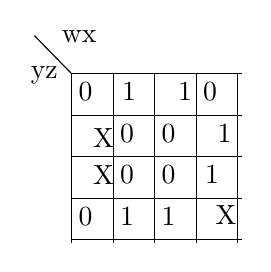
\begin{tikzpicture}[x=0.75pt,y=0.75pt,yscale=-1,xscale=1] 
\draw  [draw opacity=0] (106,41) -- (188,41) -- (188,122.6) -- (106,122.6) -- cycle ; \draw   (106,41) -- (106,122.6)(126,41) -- (126,122.6)(146,41) -- (146,122.6)(166,41) -- (166,122.6)(186,41) -- (186,122.6) ; \draw   (106,41) -- (188,41)(106,61) -- (188,61)(106,81) -- (188,81)(106,101) -- (188,101)(106,121) -- (188,121) ; \draw    ;
%Straight Lines [id:da6508935575311161] 
\draw    (88,22.6) -- (106,41) ;

% Text Node
\draw (169,84) node [anchor=north west][inner sep=0.75pt]   [align=left] {1};
% Text Node
\draw (156,44) node [anchor=north west][inner sep=0.75pt]   [align=left] {1};
% Text Node
\draw (175,64) node [anchor=north west][inner sep=0.75pt]   [align=left] {1};
% Text Node
\draw (129,44) node [anchor=north west][inner sep=0.75pt]   [align=left] {1};
% Text Node
\draw (115,66) node [anchor=north west][inner sep=0.75pt]   [align=left] {X};
% Text Node
\draw (115,84) node [anchor=north west][inner sep=0.75pt]   [align=left] {X};
% Text Node
\draw (174,103) node [anchor=north west][inner sep=0.75pt]   [align=left] {X};
% Text Node
\draw (100,19) node [anchor=north west][inner sep=0.75pt]   [align=left] {wx};
% Text Node
\draw (85,36) node [anchor=north west][inner sep=0.75pt]   [align=left] {yz};
% Text Node
\draw (148,104) node [anchor=north west][inner sep=0.75pt]   [align=left] {1};
% Text Node
\draw (128,104) node [anchor=north west][inner sep=0.75pt]   [align=left] {1};
% Text Node
\draw (108,104) node [anchor=north west][inner sep=0.75pt]   [align=left] {0};
% Text Node
\draw (128,84) node [anchor=north west][inner sep=0.75pt]   [align=left] {0};
% Text Node
\draw (148,84) node [anchor=north west][inner sep=0.75pt]   [align=left] {0};
% Text Node
\draw (148,64) node [anchor=north west][inner sep=0.75pt]   [align=left] {0};
% Text Node
\draw (128,64) node [anchor=north west][inner sep=0.75pt]   [align=left] {0};
% Text Node
\draw (108,44) node [anchor=north west][inner sep=0.75pt]   [align=left] {0};
% Text Node
\draw (168,44) node [anchor=north west][inner sep=0.75pt]   [align=left] {0};


\end{tikzpicture}

by solving above k-map we get the equation (x&&z'+x'&&z)
\section{ARDUINO CONNECTIONS}
1)Connection at breadboard
1) The connections taken from Arduino as Input and Output is as follows:
\begin{table}[ht!] 
    \centering 
    \begin{tabular}{|c|c|c|c|c|c|c|c|} 
    \hline 
       Input & $a$&$b$&$f$\\ 
       \hline 
    Arduino & 3&4&6\\ 
    \hline 
    \end{tabular} 
    \caption{} 
\end{table}
2) The  input \textbf{a,b} here are connected to Arduino D3,D4 pins.\\
3) The  output \textbf{f} here are connected to Arduino D6 pins.\\
4) The values for these inputs are conncted either to GND or 5V according to the truth table.\\
5)attaching LED' cathod to GND
\section{CODE}
\paragraph{}
	The arduino code can be downloaded from the below link.
\begin{center} 
\fbox{\parbox{8.5cm}{\url{https://github.com/madhu-addanki/FWC/tree/main/ide }}} 
\end{center}


\end{document}
